% !TEX TS-program = XeLaTeX
% use the following command:
% all document files must be coded in UTF-8
\documentclass[spanish]{textolivre}
% build HTML with: make4ht -e build.lua -c textolivre.cfg -x -u article "fn-in,svg,pic-align"

\journalname{Texto Livre}
\thevolume{16}
%\thenumber{1} % old template
\theyear{2023}
\receiveddate{\DTMdisplaydate{2022}{10}{6}{-1}} % YYYY MM DD
\accepteddate{\DTMdisplaydate{2023}{1}{22}{-1}}
\publisheddate{\DTMdisplaydate{2023}{3}{17}{-1}}
\corrauthor{Cristian Olivares-Rodríguez}
\articledoi{10.1590/1983-3652.2023.41439}
%\articleid{NNNN} % if the article ID is not the last 5 numbers of its DOI, provide it using \articleid{} commmand 
% list of available sesscions in the journal: articles, dossier, reports, essays, reviews, interviews, editorial
\articlesessionname{articles}
\runningauthor{Olivares-Rodríguez et al.} 
%\editorname{Leonardo Araújo} % old template
\sectioneditorname{Daniervelin Pereira}
\layouteditorname{Leonado Araújo}

\title{Escritura de texto y producción de código limpio: dos realidades de un mismo proceso en estudiantes de ingeniería}
\othertitle{Escrever texto e produzir código limpo: duas realidades do mesmo processo para estudantes de engenharia}
\othertitle{Text writing and clean code production: two realities of the same process in engineering students}
% if there is a third language title, add here:
%\othertitle{Artikelvorlage zur Einreichung beim Texto Livre Journal}
\author[1]{Cristian Olivares-Rodríguez \orcid{0000-0002-4991-5784} \thanks{Email: \href{mailto:cristian.olivares@uach.cl}{cristian.olivares@uach.cl}}}
\author[2,3]{Gabriel Valdés-León \orcid{0000-0001-8807-8838} \thanks{Email: \href{mailto:gabrielsebastian.valdes@ulpgc.es}
{gabrielsebastian.valdes@ulpgc.es}}}
\author[1]{Martha Vidal-Sepúlveda \orcid{0000-0002-0929-8179} \thanks{Email: \href{mailto:martha.vidal@uach.cl}
{martha.vidal@uach.cl}}}
\author[4]{Romina Oyarzún-Yañez \orcid{0000-0001-9938-6019} \thanks{Email: \href{mailto:r.amaliaoyarzun@uandresbello.edu}{r.amaliaoyarzun@uandresbello.edu}}}
\affil[1]{Universidad Austral de Chile, Instituto de informática, Facultad de Ciencias de la Ingeniería, Chile.}
\affil[2]{Universidad de Las Palmas de Gran Canaria, Facultad de Educación, España.}
\affil[3]{Universidad Bernardo O’Higgins, Centro de Investigación en Educación (CIE), Chile.}
\affil[4]{Universidad Andres Bello, Chile.}

\addbibresource{article.bib}
% use biber instead of bibtex
% $ biber article

% used to create dummy text for the template file
\definecolor{dark-gray}{gray}{0.35} % color used to display dummy texts
\usepackage{lipsum}
\SetLipsumParListSurrounders{\colorlet{oldcolor}{.}\color{dark-gray}}{\color{oldcolor}}

% used here only to provide the XeLaTeX and BibTeX logos
\usepackage{hologo}
%\usepackage[dvipsnames]{xcolor}

% if you use multirows in a table, include the multirow package
\usepackage{multirow}

% provides sidewaysfigure environment
\usepackage{rotating}

% CUSTOM EPIGRAPH - BEGIN 
%%% https://tex.stackexchange.com/questions/193178/specific-epigraph-style
\usepackage{epigraph}
\usepackage{float}

\renewcommand\textflush{flushright}
\makeatletter
\newlength\epitextskip
\pretocmd{\@epitext}{\em}{}{}
\apptocmd{\@epitext}{\em}{}{}
\patchcmd{\epigraph}{\@epitext{#1}\\}{\@epitext{#1}\\[\epitextskip]}{}{}
\makeatother
\setlength\epigraphrule{0pt}
\setlength\epitextskip{0.5ex}
\setlength\epigraphwidth{.7\textwidth}
% CUSTOM EPIGRAPH - END

% LANGUAGE - BEGIN
% ARABIC
% for languages that use special fonts, you must provide the typeface that will be used
% \setotherlanguage{arabic}
% \newfontfamily\arabicfont[Script=Arabic]{Amiri}
% \newfontfamily\arabicfontsf[Script=Arabic]{Amiri}
% \newfontfamily\arabicfonttt[Script=Arabic]{Amiri}
%
% in the article, to add arabic text use: \textlang{arabic}{ ... }
%
% RUSSIAN
% for russian text we also need to define fonts with support for Cyrillic script
% \usepackage{fontspec}
% \setotherlanguage{russian}
% \newfontfamily\cyrillicfont{Times New Roman}
% \newfontfamily\cyrillicfontsf{Times New Roman}[Script=Cyrillic]
% \newfontfamily\cyrillicfonttt{Times New Roman}[Script=Cyrillic]
%
% in the text use \begin{russian} ... \end{russian}
% LANGUAGE - END

% EMOJIS - BEGIN
% to use emoticons in your manuscript
% https://stackoverflow.com/questions/190145/how-to-insert-emoticons-in-latex/57076064
% using font Symbola, which has full support
% the font may be downloaded at:
% https://dn-works.com/ufas/
% add to preamble:
% \newfontfamily\Symbola{Symbola}
% in the text use:
% {\Symbola }
% EMOJIS - END

% LABEL REFERENCE TO DESCRIPTIVE LIST - BEGIN
% reference itens in a descriptive list using their labels instead of numbers
% insert the code below in the preambule:
%\makeatletter
%\let\orgdescriptionlabel\descriptionlabel
%\renewcommand*{\descriptionlabel}[1]{%
%  \let\orglabel\label
%  \let\label\@gobble
%  \phantomsection
%  \edef\@currentlabel{#1\unskip}%
%  \let\label\orglabel
%  \orgdescriptionlabel{#1}%
%}
%\makeatother
%
% in your document, use as illustraded here:
%\begin{description}
%  \item[first\label{itm1}] this is only an example;
%  % ...  add more items
%\end{description}
% LABEL REFERENCE TO DESCRIPTIVE LIST - END


% add line numbers for submission
%\usepackage{lineno}
%\linenumbers


\begin{document}
\maketitle

\begin{polyabstract}
\begin{abstract}
La calidad de los productos de software depende en gran medida de la capacidad de los desarrolladores de generar código limpio, puesto que permiten incrementar el ciclo de vida del software. Por ello, resulta crucial mejorar las prácticas pedagógicas de la enseñanza de la programación, en particular, la capacidad de escribir código de calidad por parte de los estudiantes. Sin embargo, en la literatura no se reconocen modelos pedagógicos integrales que guíen el desarrollo de esta capacidad de escritura, tal como se observa en la escritura de textos. El objetivo de este trabajo es relacionar la producción de código limpio con las concepciones sobre el proceso de escritura en estudiantes de Ingeniería Informática. Para ello, se diseñaron tres evaluaciones prácticas que permitieron acompañar el proceso de programación de código limpio de los estudiantes universitarios para, posteriormente, relacionar los resultados con las percepciones sobre la escritura que este grupo posee. Dentro de los principales resultados, destaca la relación entre el rendimiento en las tareas de programación y el año de ingreso, así como la correlación positiva entre la producción de código limpio y las concepciones sobre la escritura. Esto abre un espacio inexplorado de colaboración transdisciplinar que permita avanzar hacia un modelo pedagógico que dirija la enseñanza de la escritura de código limpio que contribuya con productos de software de mayor calidad.

\keywords{Programación computacional \sep Escritura \sep Educación en Ingeniería}
\end{abstract}

\begin{portuguese}
\begin{abstract}
A qualidade dos produtos de \textit{software} depende em grande parte da capacidade dos desenvolvedores de gerar código limpo, uma vez que eles permitem aumentar o ciclo de vida do \textit{software}. Portanto, é crucial melhorar as práticas pedagógicas de ensino de programação, em particular, a capacidade dos estudantes de escrever código de qualidade. Entretanto, a literatura não reconhece modelos pedagógicos abrangentes que orientam o desenvolvimento dessa capacidade de escrita, como observado na redação de textos. Este trabalho relaciona a produção de código limpo com as concepções do processo de escrita em estudantes de Engenharia da Computação. Para esse fim, utilizamos três avaliações práticas para avaliar o processo de programação de código limpo em estudantes universitários, para, posteriormente, relacionar os resultados com as percepções sobre a escrita que esse grupo tem. Os resultados mostram uma relação entre o desempenho nas tarefas de programação e o ano de ingresso, e uma correlação positiva entre a produção de código limpo e as concepções sobre a escrita. Concluímos que nosso estudo abre uma colaboração transdisciplinar. Ele pode avançar em direção a um modelo pedagógico para orientar o ensino da escrita limpa de código que contribui para produtos de \textit{software} de maior qualidade.

\keywords{Programação de computadores \sep Linguagem escrita \sep Educação em engenharia}
\end{abstract}
\end{portuguese}

\begin{english}
\begin{abstract}
The quality of software products depends to a large extent on the ability of developers to generate clean code since they allow increasing the software life cycle. Therefore, it is crucial to improve the pedagogical practices of teaching programming, in particular, the ability of students to write quality code. However, the literature does not recognize comprehensive pedagogical models that guide the development of this writing ability, as observed in text redaction. This paper relates the production of clean code with the conceptions of the writing process in Computer Engineering students. Thereby, we used three practical assessments to evaluate the process of clean code programming on university students to later relate the results with the perceptions about writing that this group has. Results show a relationship between performance in programming tasks and the cohort and a positive correlation between the production of clean code and conceptions about writing. We conclude that our study opens a transdisciplinary collaboration. It can advance towards a pedagogical model to guide the teaching of clean code writing that contributes to higher quality software products.

\keywords{Computer programming \sep Written language \sep Engineering education}
\end{abstract}
\end{english}
% if there is another abstract, insert it here using the same scheme
\end{polyabstract}

\section{Introducción}\label{sec-intro}
% Problema
La calidad del producto de software se sustenta, principalmente, en la capacidad de producir código limpio. Un código limpio contribuye con la escalabilidad, reutilización y optimización de las componentes de software del producto construido. Sin embargo, observamos que el principal desafío es integrar estos aspectos técnicos avanzados con una mayor sistematización pedagógica, contribuyendo con la calidad de los productos desarrollados en contextos universitarios, en concreto, a su estabilidad y continuidad del proceso de negocio soportado por el servicio tecnológico. Esto no debe dejar de lado la complejidad observada en los cursos introductorios de programación \cite{figueiredo2022strategies}.

%Motivación
La motivación de este estudio radica en el cambio cultural de las actuales fábricas de software, las que se encuentran en un tránsito desde la centralización de las tareas de aseguramiento de la calidad en metodologías rígidas a la distribución de las responsabilidades de la producción desde etapas tempranas en metodologías ágiles. Para ello, es necesario distribuir el trabajo y responsabilidades entre los miembros del equipo. De esta manera, cobra relevancia la formación en competencias de trabajo en equipo, colaboración y en la producción de código limpio que permitan la integración continua y una fácil lectura por cada uno de los desarrolladores que forman o formarán parte de un equipo.


%Objetivo
El objetivo de esta investigación es relacionar la producción de código limpio con las concepciones sobre el proceso de escritura en estudiantes de Ingeniería informática. De este objetivo, se desprende nuestro interés por poner en diálogo el mundo de la escritura “tradicional” con el de la producción de código informático, lo que nos lleva a indagar en torno a una eventual correlación entre estas dos variables. El valor de esto radica en que, de corroborarse un vínculo entre ellas, sería posible revisitar las décadas de investigación en cuanto a la didáctica de la escritura con el fin de aplicar estos avances en el ámbito de la enseñanza de la programación. 

%Contribución
 La principal contribución de este estudio es la habilitación del camino hacia nuevas prácticas pedagógicas para la enseñanza de la producción de código limpio en estudiantes universitarios, dada la positiva relación observada entre la producción de código limpio y las percepciones de escritura. Asimismo, en el diseño de nuevas prácticas es imprescindible integrar las habilidades y percepciones de escritura/lectura de textos. 

 
%Adicionalmente,  Es decir, el valor de los nuevos equipos de desarrollo está en las personas que producen software de calidad en directa colaboración con el cliente para abordar los cambios de manera temprana, distribuyendo el trabajo y responsabilidades entre los miembros del equipo. Desde esta perspectiva, el producto de software devenido en medio de comunicación es la interfaz entre desarrolladores y entre el cliente y los usuarios. Sumado a esto, la enseñanza del software también es responsable de cumplir con el código de ética de la ingeniería de software propuesto por la ACM, en particular, a los principios de responsabilidad profesional. De esta manera, cobra relevancia la formación en competencias de trabajo en equipo, colaboración y en la producción de código limpio que permitan la integración continua y una fácil lectura por cada uno de los desarrolladores que forman o formarán parte de un equipo. 



\section{Trabajos relacionados}
La producción de código limpio implica la reducción y/o eliminación de los \textit{code smells} que emergen de las primeras versiones del producto, ya que son los principales responsables de la reducción de la calidad del producto de software. Estos \textit{code smells} están directamente vinculados con los posibles fallos futuros del software dificultando la capacidad de mantención del producto, lo que se traduce en limitaciones en la calidad del servicio del negocio en el cual se inserta el desarrollo. 

Los \textit{code smells} son síntomas observables o anomalías que emergen durante el proceso de escritura del código y, por tanto, limitan la evolución del producto de software debido a que complejizan su lectura. Se ha propuesto este término para referirse a patrones que contienen problemas estructurales observables en el código que deberían ser mejorados \cite{fowler2018refactoring}. Desde la conceptualización de Fowler y sus colegas, se han propuesto diferentes listas de identificación y organización de \textit{code smells} en los productos de software. Se han identificado antipatrones de desarrollo, los cuales integran elementos arquitectónicos, de desarrollo y de gestión que se traducen en consecuencias negativas para el producto \cite{brown1998architectures}. Asimismo, se han identificado \textit{code smells} con el propósito de vincularlos con técnicas de \textit{refactoring} pertinentes para dichos síntomas \cite{fowler2018refactoring, lacerda2020code}. Estas listas han sido complementadas con nuevas categorías de problemas que han sido capturados desde la práctica profesional \cite{gupta2016modelling} o extendidas a antipatrones presentes en productos basados en patrones arquitectónicos comúnmente utilizados en la industria del software, tal como el modelo MVC \cite{aniche2018code} o extendidas a tipos de productos en particular, tales como los desarrollos de productos de \textit{machine learning} \cite{van2021prevalence, liu2019deep}. 

\subsection{La enseñanza de código limpio}
La programación es el proceso de resolución de problemas a través de algoritmos computacionales, que corresponden a una secuencia de instrucciones que permiten dar respuesta a una necesidad de información por medio de la implementación sobre un lenguaje de programación apropiado al contexto. Por lo tanto, la enseñanza de la programación debe ser abordada desde la perspectiva del pensamiento computacional \cite{wing2008computational, voogt2015computational}, contemplando el desarrollo de la capacidad de resolución de problemas computacionales, entendida como un abordaje metodológico que busca comprender las necesidades de información en el dominio del problema, extraer la información relevante del dominio por medio de abstracciones en el espacio de solución y establecer una secuencia lógica que resuelva el problema. 

El proceso de análisis abstracto debe llegar a ser implementado de manera concreta, por medio de la escritura de código, en un lenguaje de programación. Esto impondrá restricciones a la solución diseñada en función de su paradigma y estructura sintáctica. Mientras que  el paradigma de programación establece las reglas de composición de las piezas de código, la sintaxis define las reglas de escritura del lenguaje. Este proceso de comprensión del problema y creación de soluciones interactúa tanto con el pensamiento crítico \cite{bastias2021evaluation}, en la evaluación del problema; como con el pensamiento creativo, durante la evaluación de las alternativas de solución \cite{eguiluz2017exploring, groeneveld2022undergraduate}. En consecuencia, los programadores deben ser capaces de resolver problemas por medio de la escritura de código o codificación, ajustándose a las reglas del lenguaje sobre el cual se escribe para establecer una solución apropiada y de calidad. 

Por lo tanto, los cursos de programación en la educación superior, principalmente en los programas de estudio asociados a las ciencias de la computación, se orientan a desarrollar la capacidad de escribir código que permita resolver problemas simples y se estructuran en torno a dos ejes formativos: la resolución de problemas o nivel abstracto; y la comprensión lenguaje de programación o nivel operativo \cite{iqbal2021web}. De esta manera, se han propuesto diversos acercamientos pedagógicos que dependen del énfasis con el cual se combinan estos ejes. 

En particular, para el desarrollo de las habilidades de programación se han propuesto una serie de prácticas pedagógicas que apuntan a mejorar la calidad del código generado por los estudiantes. Más allá de la selección del lenguaje de programación, la orientación pedagógica ha delineado dos tipos de prácticas: 1) la lectura de código y 2) la escritura de código; tendiendo en consideración que ambas habilidades se encuentran estrechamente relacionadas. 

Una de las principales prácticas pedagógicas en la enseñanza de la programación es la escritura de código. Esta se centra en la formación de habilidades técnicas asociadas al lenguaje de programación y la capacidad de los estudiantes para establecer una secuencia algorítmica desde el análisis abstracto. \textcite{fincher1999we} describe cuatro acercamientos metodológicos para la enseñanza de la programación enfocados en las capacidades de análisis de los aprendices antes de avanzar en la codificación. Esto se encuentra alineado con las propuestas actuales basadas en la programación por bloques \cite{kyfonidis2017block, weintrop2019block}, lo que reduce la complejidad en la adquisición del lenguaje y se enfoca en la capacidad de abstracción. Sin embargo, la estrategia pedagógica clásica es la de sesiones teóricas seguidas de prácticas, autónomas o guiadas \cite{murphy2016analysis}. Mientras que los principales lenguajes de programación son Java y, actualmente, Python \cite{becker201950}, lo que puede estar relacionado con sus características de tipado débil. Sin embargo, estas prácticas apuntan a la formación en cursos introductorios, donde los estudiantes deben comprender el proceso de resolución de problemas por medio de algoritmos computacionales.

Mientras que, por otra parte, la lectura de código como práctica pedagógica aborda el fomento de la codificación limpia por medio de la capacidad de análisis de la sintaxis del lenguaje de programación y las semánticas de las soluciones escritas previamente. Por consiguiente, la introducción de \textit{bugs} en códigos ha sido utilizada como práctica pedagógica, reflejando que los estudiantes que reciben este tipo de códigos mal escritos alcanzan mejores resultados de aprendizaje que sus pares \cite{griffin2019designing}. Similarmente, la enseñanza del código limpio desde la lectura está dirigida por la retroalimentación oportuna, la cual comienza por sesiones teórico-prácticas de lectura de código de manera interactiva, sesiones de revisión de tareas en directo con los estudiantes y la evaluación individual y oral de las competencias de codificación limpia \cite{dietz2018teaching}. Mientras que otro estudio aborda el diseño de un tutor inteligente que presenta a los estudiantes trozos de código de baja calidad para evaluar su calidad, contribuyendo con la capacidad de producción código limpio \cite{prokic2021clean}. Por lo tanto, la capacidad de lectura de códigos influye positivamente en la capacidad de escritura de los educandos. Esta relación trae consigo, de manera implícita, que la capacidad de producción de código limpio se encuentra ligada a la capacidad de lectura de código debido al fomento del proceso reflexivo y analítico que trae consigo la exploración de trozos de código.

\subsection{Concepciones sobre el proceso de escritura}

Durante los últimos años, los estudios sobre escritura en la educación terciaria han tenido un aumento exponencial \cite{navarro2016panorama}. Mucha tinta se ha vertido en relación con la importancia de acompañar el proceso de alfabetización académica de los estudiantes universitarios con énfasis en los de nuevo ingreso \cite{roald2021learning}, quedando en segundo plano las investigaciones realizadas con alumnos de nivel de posgrado \cite{calle2022obstacles}.

Lo anterior se justifica debido a la importancia que tiene la escritura en la formación universitaria, principalmente en los primeros años, e independiente del área epistémica. Diversos son los estudios que establecen una estrecha relación entre el éxito académico y las competencias comunicativas productivas \cite{ulu2019investigation, turkben2021relationship} y receptivas \cite{kilner2019using, liu2020general}, pero, además, su importancia en el crecimiento disciplinar de los aprendientes.

Al respecto, autores como \textcite{walton2020writing} o \textcite{selwyn2020developing} destacan la importancia del dominio de estas habilidades para los estudiantes y profesionales de la ingeniería, pero, al mismo tiempo, dan cuenta de que su desarrollo es aún un desafío pendiente. En palabras de \textcite[p. 71]{goldsmith2019investigating}:

\begin{quote}
Much has been written about the importance of getting engineering students to write, but there has been a little investigation of engineering academics’ perceptions of writing practices in the curriculum, and the extent to which these practices are visible to their students and to the academics. 
\end{quote}

La presente investigación se enfoca, precisamente, en el campo de los estudios sobre las concepciones que tienen los aprendientes sobre la escritura, debido a que uno de los ámbitos que resulta más enriquecedor para los actores del proceso educativo es el de las percepciones en torno a la escritura. Esto se debe a que el manejo de esta información permite acompañar de manera efectiva los procesos de enseñanza, pues se ha comprobado que existe una estrecha relación entre las concepciones de la escritura y los resultados de aprendizaje, tal como señalan \textcite{miras2013creencias} en el nivel secundario o \textcite{gonzalez2020concepciones} en el nivel terciario, por nombrar un par de ejemplos.

Al abordar las concepciones en torno a la escritura, distintas son las perspectivas que podemos adoptar. Por ejemplo, algunas investigaciones indagan en cómo conciben los estudiantes la escritura, vale decir, si valoran su dimensión epistémica o se quedan simplemente con su función reproductiva \cite{gonzalez2020concepciones}. Por su parte autores como \cite{lonka2014measure} se interesan en un mayor número de aspectos, muchos de ellos relacionados con el proceso de escritura: bloqueos, procrastinación, perfeccionismo, habilidad innata, transformación del conocimiento y productividad. Ahora bien, para los fines de nuestra investigación, hemos adoptado la propuesta de \textcite{vine2020escritura}, pues se enfoca, específicamente, en el proceso de escritura. La autora, sobre la base de los trabajos de \textcite{de2012hacia} o \textcite{rodriguez2015escritura}, aborda las tres instancias del proceso de escritura (antes, durante y después) a través de cinco dimensiones: planificación, textualización, revisión, postergación del inicio de la escritura y actitudes hacia la escritura. 

\section{Materiales y métodos}

El trabajo ha sido diseñado como un estudio transversal, pues la información fue recogida en un único momento. Asimismo, posee carácter descriptivo, ya que busca conocer cómo operan las dos variables consideradas en una situación particular. Por último, posee un alcance correlacional, debido a que entrega un explicación -parcial, por cierto- al fenómeno estudiado.

\subsection{Participantes}

Participaron de la investigación 28 estudiantes de la asignatura de ingeniería de software de Ingeniería civil en informática. Se seleccionó dicha muestra debido a la estrecha relación entre la investigación y el objetivo principal del curso.  Específicamente, esta asignatura tiene como objetivo que los estudiantes sean capaces de desarrollar productos de software usables y de calidad por medio de métodos sistemáticos utilizados en la industria del software. Por lo tanto, es necesario que apliquen las habilidades de resolución de problemas y de escritura de código adquiridas en los primeros años de la carrera de manera guiada. Asimismo, en la asignatura se revisan los siguientes contenidos técnicos: 
\begin{enumerate*}[label=\arabic*)]
    \item Metodologías de desarrollo de software,
    \item Codificación limpia y
    \item Calidad de software.
\end{enumerate*}


\subsection{Protocolo experimental}

Para alcanzar el objetivo se planteó un estudio relacional cuasi-experimental en la asignatura de ingeniería de software. En la \Cref{fig-metodo} se presenta el protocolo experimental utilizado en este estudio.

\begin{figure}[H]
\centering
\begin{minipage}{0.75\textwidth}
 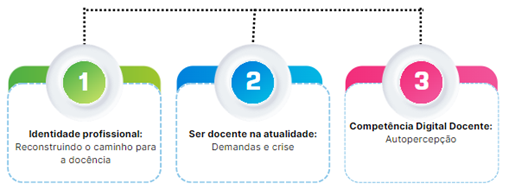
\includegraphics[width=\textwidth]{figuras/Figura1.png}
 \caption{Protocolo cuasi-experimental.}
 \label{fig-metodo}
 \source{Elaboración propia.}
\end{minipage}
\end{figure}


\subsection{Instrumentos de evaluación del producto de software}

Para evaluar la capacidad de desarrollo de software adquiridas por los participantes tanto en la asignatura intervenida como en los primeros años de la carrera, se aplicaron tres evaluaciones prácticas basadas en la resolución de 3 casos de estudios reales. 

\begin{itemize}
    \item \textbf{Evaluación 1 “Metodologías de resolución de problemas”}: En la primera actividad evaluativa, los estudiantes debían establecer los límites del problema a resolver y planificar una estrategia de resolución por medio de un producto de software. Al respecto, era indispensable que establecieran las abstracciones necesarias para su implementación en un entorno de desarrollo web. Esta actividad consideraba:
    \begin{itemize}
        \item Análisis del problema.
        \item Modelado de la solución.
        \item Planificación del proyecto.
    \end{itemize}
    \item \textbf{Evaluación 2 “Codificación limpia”}: En la segunda actividad evaluativa, los estudiantes debían establecer un modelado arquitectónico de la solución, considerando la aplicación de patrones de diseño y buenas prácticas de codificación. En esta oportunidad, los estudiantes debían implementar la solución de manera modular en un lenguaje de programación web, considerando lo siguiente:
    \begin{itemize}
        \item Patrones de diseño.
        \item Pruebas unitarias.
        \item \textit{Code smells}.
        \item Refactorización.
    \end{itemize}
    \item \textbf{Evaluación 3 “Arquitecturas limpias”}: En la última actividad evaluativa, los estudiantes debían realizar una estimación del esfuerzo y costo del desarrollo de un producto de software y, además, implementar uno de los módulos del producto. En esta ocasión, se consideraban las siguientes actividades:
    \begin{itemize}
        \item Estimación del producto de software.
        \item Modelado arquitectónico limpio.
        \item Codificación limpia.
    \end{itemize}
\end{itemize}

\subsection{Instrumento de percepción del proceso de escritura}

Las percepciones sobre el proceso de escritura fueron recogidas por medio del cuestionario propuesto por \textcite{vine2020escritura}, el que fue diseñado a partir de los trabajos de \textcite{de2012hacia} y \textcite{rodriguez2015escritura}. 
Este cuestionario de 36 preguntas evalúa cinco dimensiones: planificación, textualización, revisión, postergación del inicio de la escritura y actitudes hacia la escritura. Se optó por este instrumento debido a que recoge información tanto del proceso como de las actitudes relacionadas con la escritura y, además, porque fue diseñado e implementado por la autora para ser aplicado en el contexto chileno, lo que da cuenta de su pertinencia cultural. La autora comparte el instrumento, de manera íntegra, en \cite{vine2020escritura}.% VINE-JARA (2020).

Finalmente, en relación con la fiabilidad del cuestionario, el coeficiente de alfa de Cronbach se observa en la \Cref{fiabilidad}, lo que permite observar que el instrumento posee una alta consistencia interna.

\begin{table}[htpb]
\centering
\begin{threeparttable}
\caption{Fiabilidad del cuestionario por dimensión.}
\label{fiabilidad}
\begin{tabular}{ll}
\toprule 
Dimensión & Alfa de Cronbach \\ 
\midrule
Planificación & 0,82\\
Textualización & 0,67\\
Revisión & 0,79\\
Postergación & 0,68\\
Actitudes & 0,76\\
\bottomrule
\end{tabular}
\source{Elaboración propia.}
\end{threeparttable}
\end{table}

\section{Resultados}

A continuación, se presentan los resultados del estudio exploratorio experimental desarrollado en el curso de Ingeniería de Software. En primer lugar, se presentan los niveles de logro alcanzados por los estudiantes en las evaluaciones formativas de la asignatura. En segundo lugar, se presentan las distribuciones en la concepción del proceso de escritura. Y, finalmente, se presentan las relaciones entre el desempeño académico en la producción de software y la concepción de la escritura.

\subsection{Desempeño académico}

Durante el primer mes del periodo lectivo, se analizaron diversas estrategias metodológicas utilizadas en la resolución de problemas por medio de la producción de productos de software. Una de las principales competencias a desarrollar es el análisis del dominio del problema, reconociendo los factores externos e internos de la organización para identificarlo apropiadamente. Esto permite a los estudiantes establecer una estrategia coherente con el contexto del problema, diseñando las acciones que deberán ser llevadas a cabo durante el proceso de producción de software. De esta forma, en la primera evaluación práctica, los estudiantes debían resolver como caso de estudio una licitación pública. 

La \Cref{fig-eval1} corresponde a la distribución de calificaciones de los estudiantes en la primera evaluación de la asignatura (eje vertical), organizados por año de ingreso (eje horizontal). En ella se observa una relación entre la cohorte y el desempeño observado en las estrategias diseñadas para resolver los problemas. Así, los estudiantes que ingresaron en el año 2018 y 2019 tienden a alcanzar mejores resultados, con una media en torno al 4.5 sobre 7.0. Mientras que los estudiantes de generaciones anteriores tienen una media en torno al 3.8, considerando un 4.0 la calificación mínima para aprobar la evaluación. En consecuencia, se observa que el desempeño se encuentra estrechamente influenciado por el año de ingreso de los estudiantes, lo que podría asociarse al desempeño general de las nuevas generaciones en el programa de estudios.

\begin{figure}[H]
\centering
\begin{minipage}{.75\textwidth}
 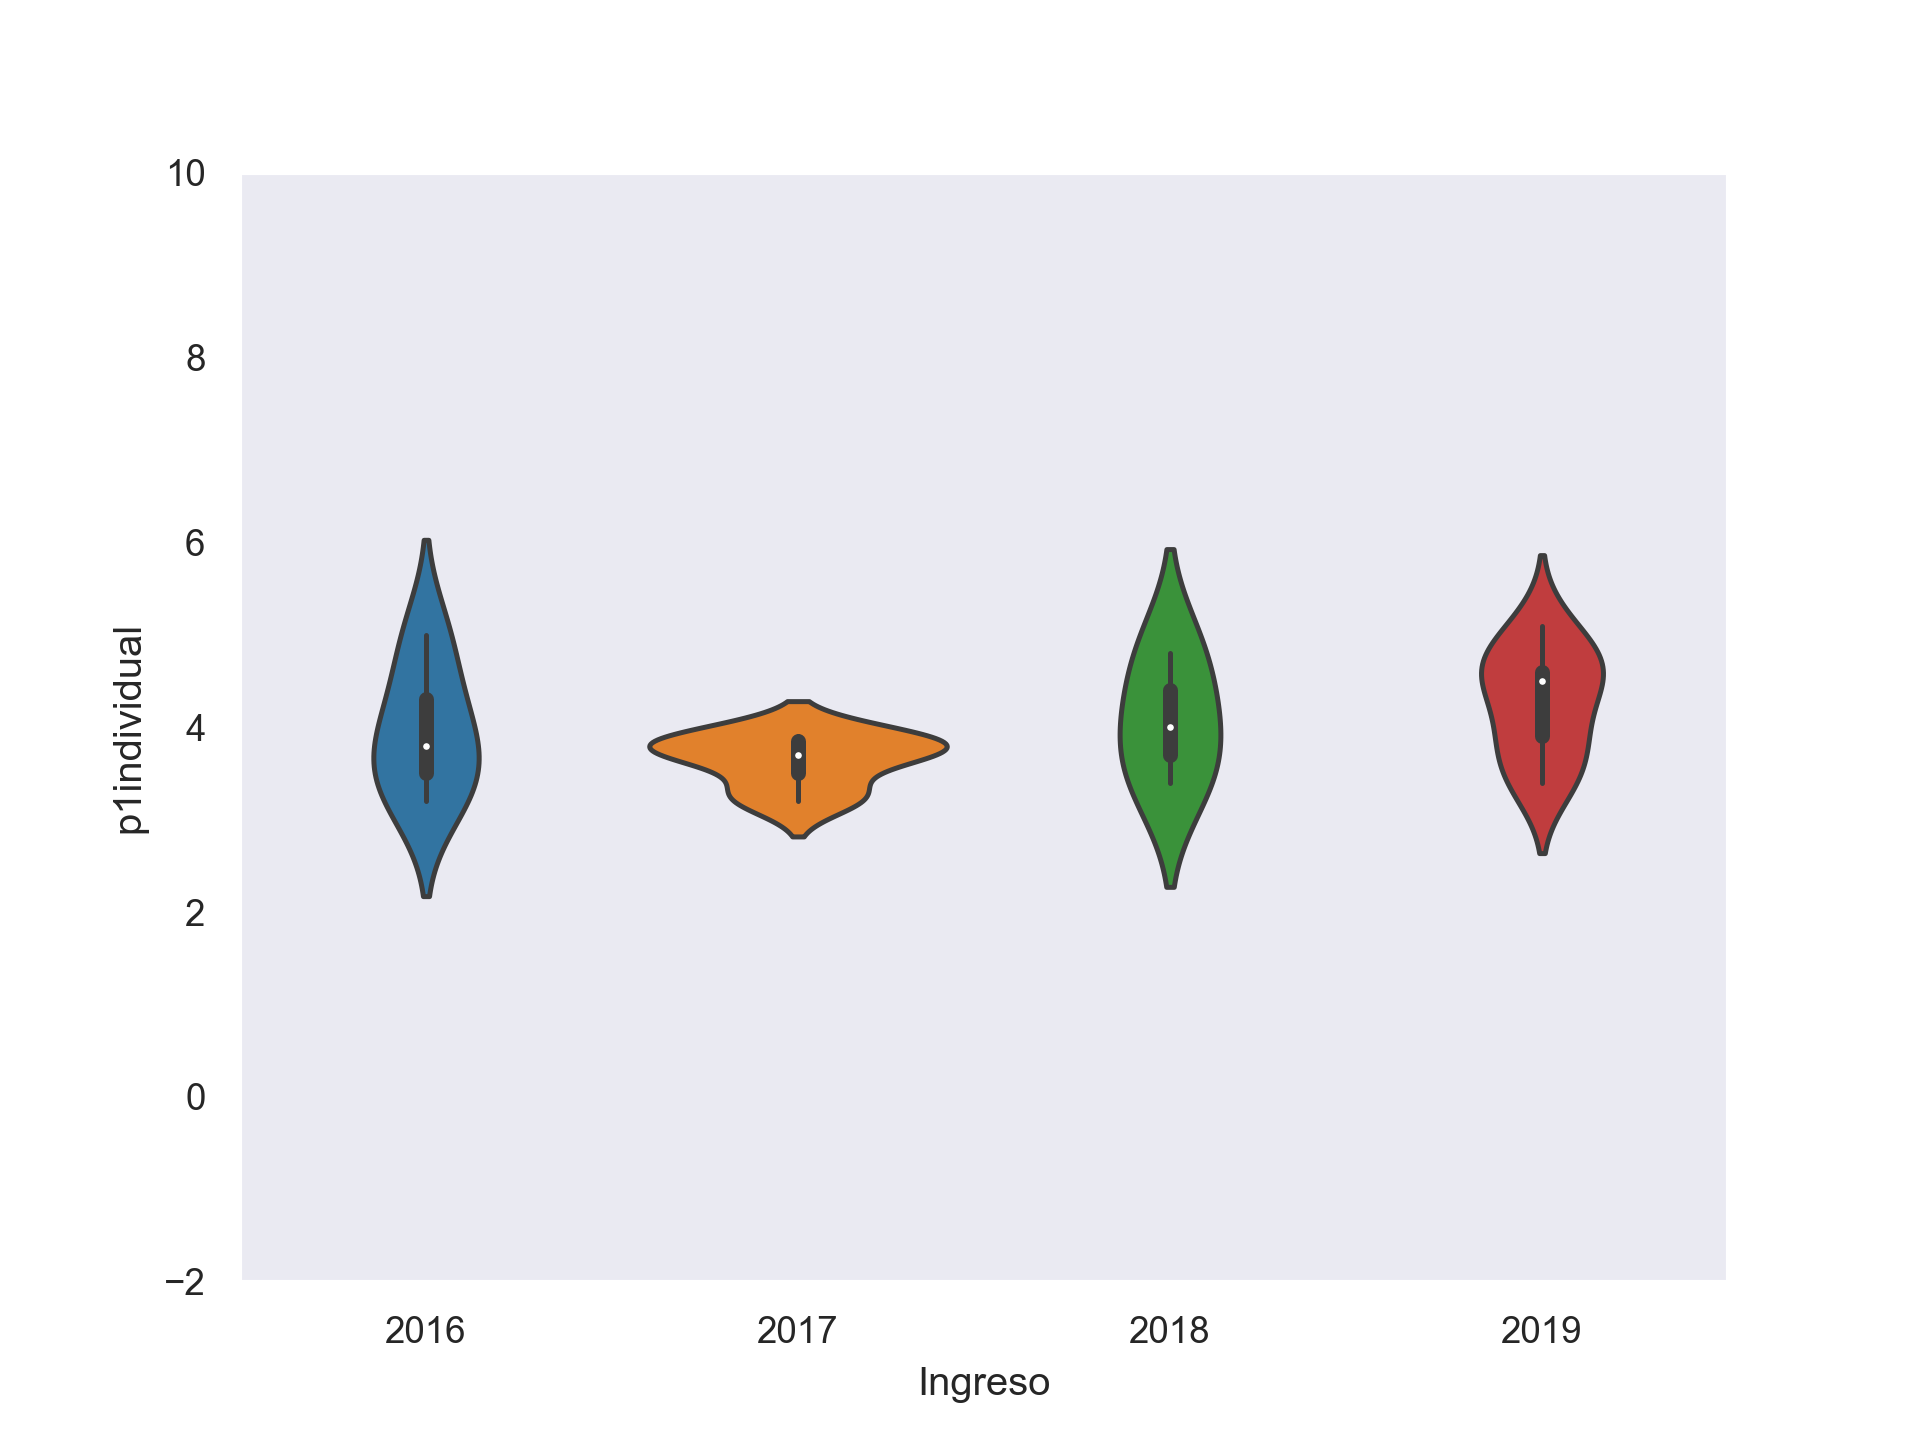
\includegraphics[width=\textwidth]{figuras/figura2.png}
 \caption{Desempeño en la primera evaluación “Metodologías de resolución de problemas”, según año de ingreso.}
 \label{fig-eval1}
 \source{Elaboración propia.}
\end{minipage}
\end{figure}

Durante el segundo mes y medio del periodo lectivo, se analizaron diversos enfoques para la producción de código limpio. En primer lugar, se revisaron los principales tipos de patrones de diseño tanto de manera abstracta como aplicados a diferentes lenguajes de programación. Luego, se revisaron estrategias de refactorización dirigidas por la identificación de \textit{code smells} para mejorar la calidad de la producción de código. Finalmente, se revisaron estrategias de diseño e implementación de pruebas para guiar el proceso de mejora de la calidad del código, tanto a nivel de componentes como de manera integral. En la segunda evaluación práctica, los estudiantes debían resolver una nueva licitación pública codificando una de las componentes diseñadas. 

La \Cref{fig-eval2} corresponde a la distribución de calificaciones de los estudiantes en la segunda evaluación de la asignatura (eje vertical), organizados por año de ingreso (eje horizontal). Nuevamente se aprecian diferencias entre generaciones, donde los estudiantes que ingresaron en los años 2018 y 2019 logran un mejor desempeño, con una media de 4.8. Mientras que las generaciones mayores alcanzan calificaciones en torno al 3.3, considerando que la aprobación se logra sobre el 4.0. Por lo tanto, en esta segunda calificación se repite la relación entre la cohorte y el desempeño académico logrado por los participantes.

\begin{figure}[H]
\centering
\begin{minipage}{.75\textwidth}
 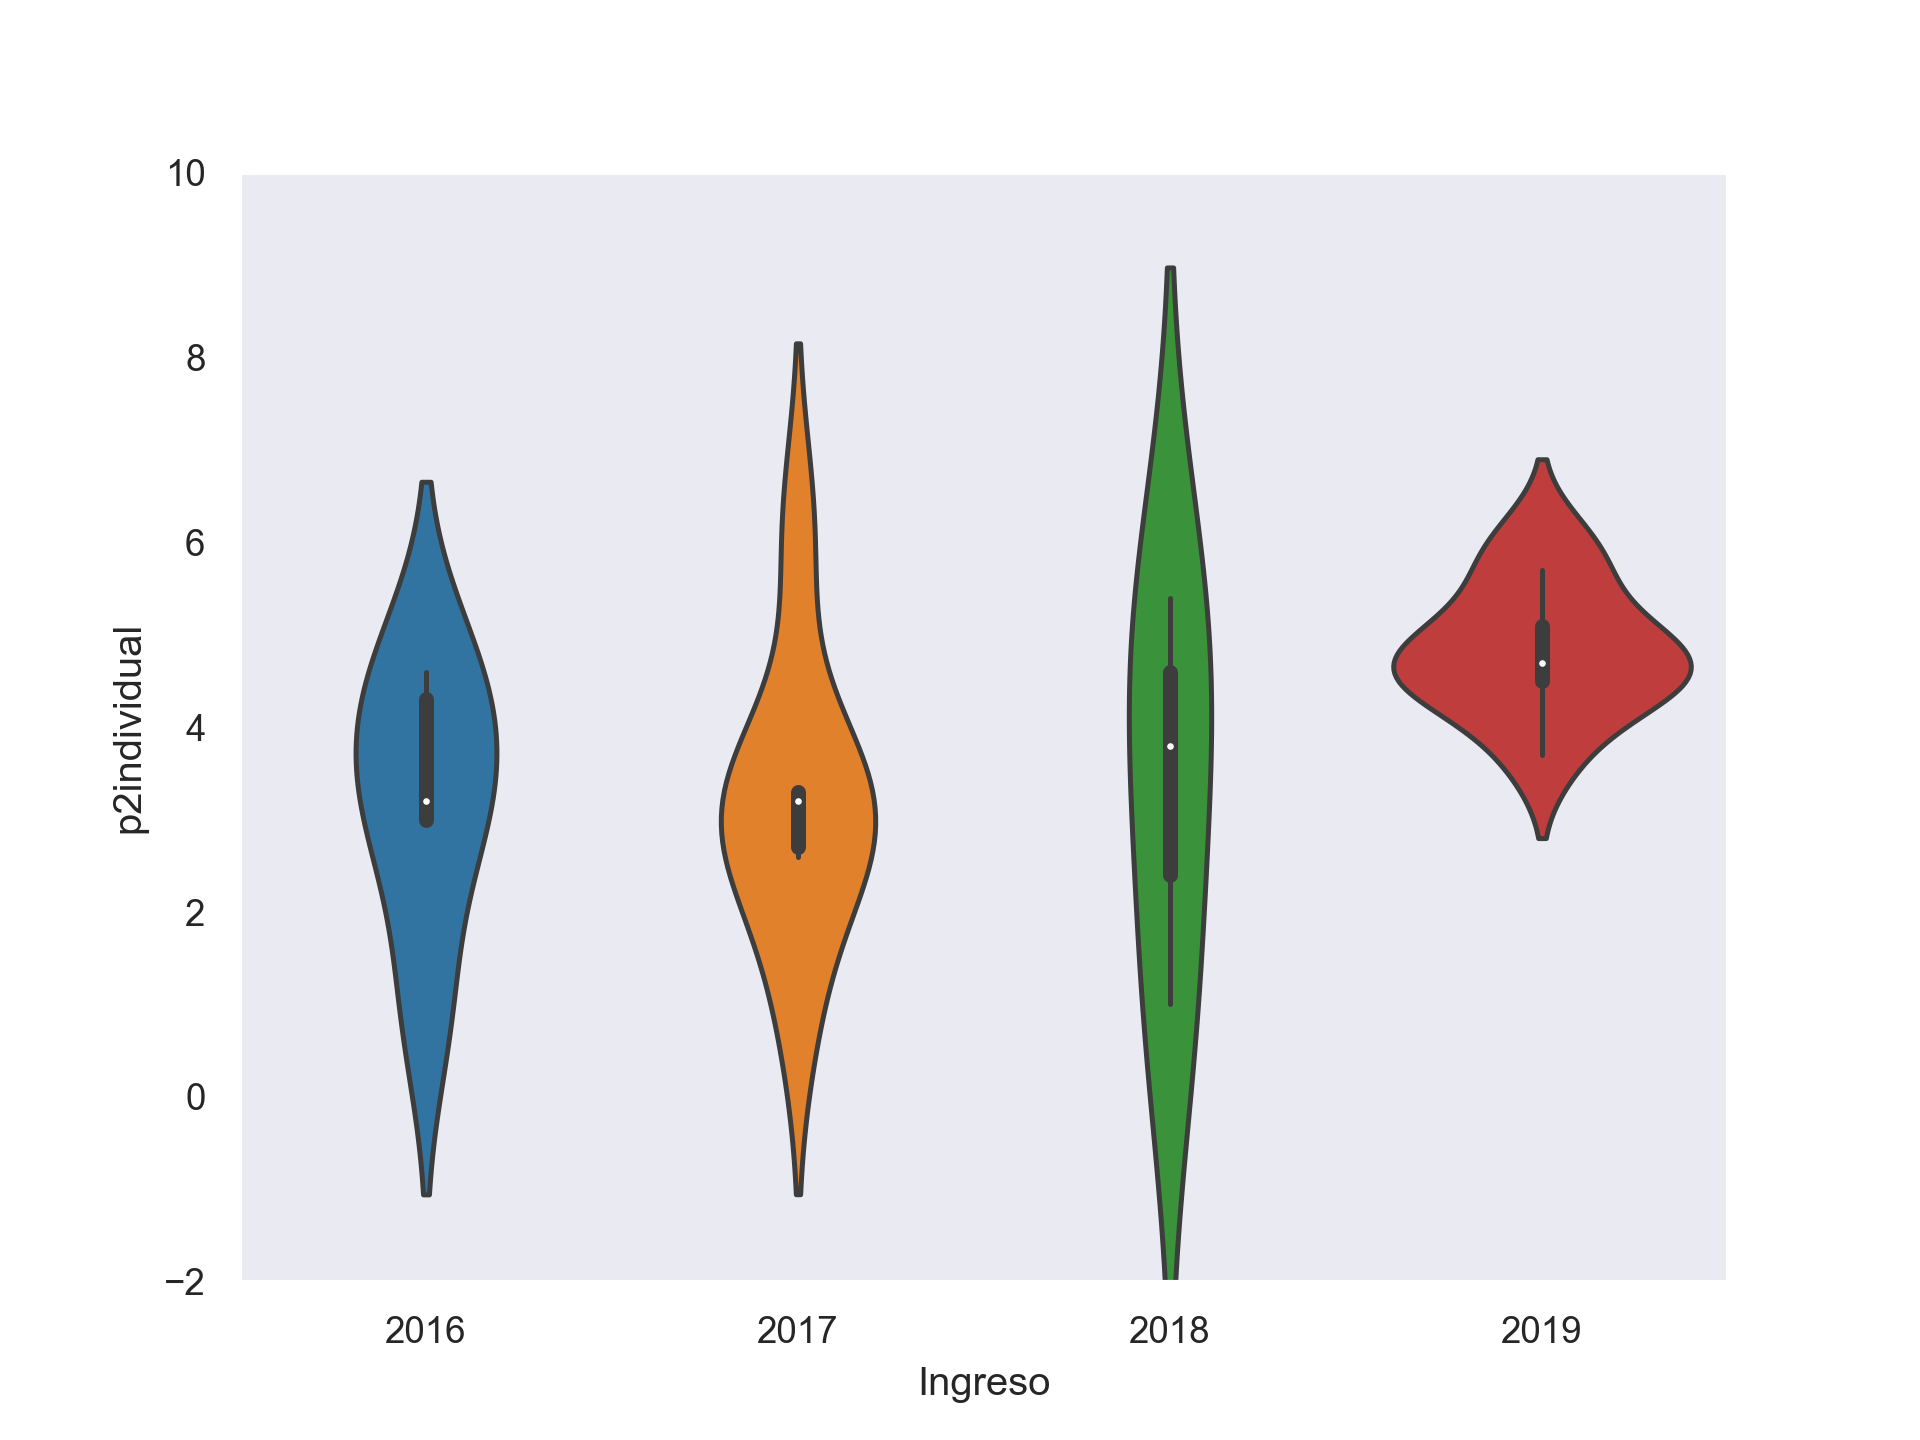
\includegraphics[width=\textwidth]{figuras/figura3.png}
 \caption{Desempeño en la segunda evaluación “Codificación limpia”, según año de ingreso.}
 \label{fig-eval2}
 \source{Elaboración propia.}
\end{minipage}
\end{figure}

Durante el último tramo del periodo lectivo, se analizaron diversas estrategias de estimación del tamaño, esfuerzo y costo del proceso de producción de software, las que dependen del paradigma de los lenguajes de programación, el contexto del problema y la arquitectura seleccionada. Para ello, se revisaron modelos de estimación de proyectos de software, desde los más simples hasta los más complejos. Además, se revisaron las implicancias que tienen las arquitecturas limpias tanto en la producción como en la mantención de productos de software. En la tercera evaluación práctica, los estudiantes debían resolver una nueva licitación pública, codificando una de las componentes de la arquitectura limpia diseñada y utilizada para la estimación del producto de software.

La \Cref{fig-eval3} corresponde a la distribución de calificaciones de los estudiantes en la segunda evaluación de la asignatura (eje vertical), organizados por año de ingreso (eje horizontal). Nuevamente se observa la relación entre la cohorte de los estudiantes y el desempeño académico, donde los estudiantes de las nuevas cohortes alcanzan calificaciones en torno al 5.2. Mientras que las cohortes anteriores tienden a obtener calificaciones menores en torno al 3.3, considerando que la aprobación se alcanza con un 4.0. Por lo tanto, en esta tercera calificación se reafirma la relación entre la cohorte y el desempeño académico logrado por los participantes.

\begin{figure}[H]
\centering
\begin{minipage}{.9\textwidth}
 
\includegraphics[width=.8\textwidth]{figuras/figura4.png}
 \caption{Desempeño en la tercera evaluación “Arquitecturas limpias”, según año de ingreso.}
 \label{fig-eval3}
 \source{Elaboración propia.}
\end{minipage}
\end{figure}

\subsection{Concepción de la escritura}

El instrumento utilizado para medir las concepciones sobre la escritura tiene la ventaja de que no solo considera las etapas de este proceso, sino que también entrega información valiosa en torno a las actitudes de los estudiantes en relación con la escritura, y sobre una de las mayores dificultades de los estudiantes al momento de redactar: la dilación del inicio de la escritura. En la \Cref{fig-concepciones}, se observa que, en términos generales, los resultados tienden a agruparse con una leve tendencia negativa, sobre todo, en las dimensiones de textualización y de postergación. Por su parte, las etapas de planificación y de revisión se presentan como aquellas con mejores resultados.

\begin{figure}[H]
\centering
\begin{minipage}{.75\textwidth}
 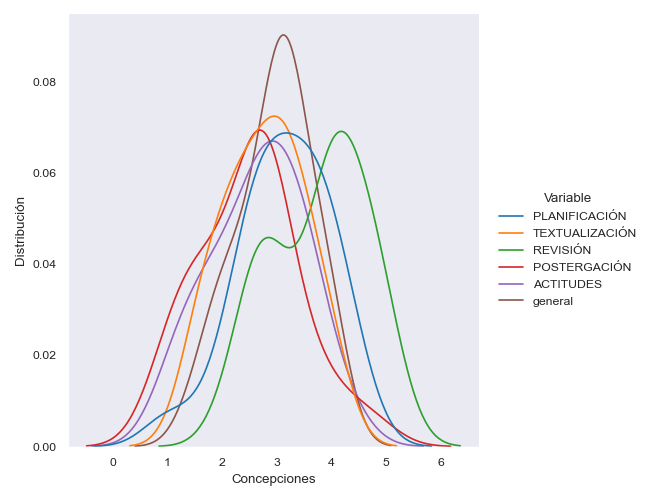
\includegraphics[width=\textwidth]{figuras/figura5.png}
 \caption{Distribución de concepciones del proceso de escritura, según dimensiones.}
 \label{fig-concepciones}
 \source{Elaboración propia.}
\end{minipage}
\end{figure}

Tal como señalamos con anterioridad, se observaron resultados interesantes al momento de organizar los datos obtenidos por año de ingreso. En el caso de las percepciones sobre la escritura, en la \Cref{fig-percepcion}, se presentan los niveles de percepción de la escritura (eje vertical) en relación al año de ingreso a la universidad (eje horizontal). En ella se vislumbran mejores resultados en la cohorte 2016, seguida de la perteneciente al 2019. Sin embargo, lo verdaderamente llamativo corresponde a la distribución de la cohorte 2017, pues da cuenta de un alto nivel de dispersión en sus resultados. Al comparar este gráfico con el correspondiente al desempeño en codificación limpia (\Cref{fig-eval2}), se observa un alto grado de similitud con los datos obtenidos en la segunda evaluación.

\begin{figure}[H]
\centering
\begin{minipage}{.75\textwidth}
 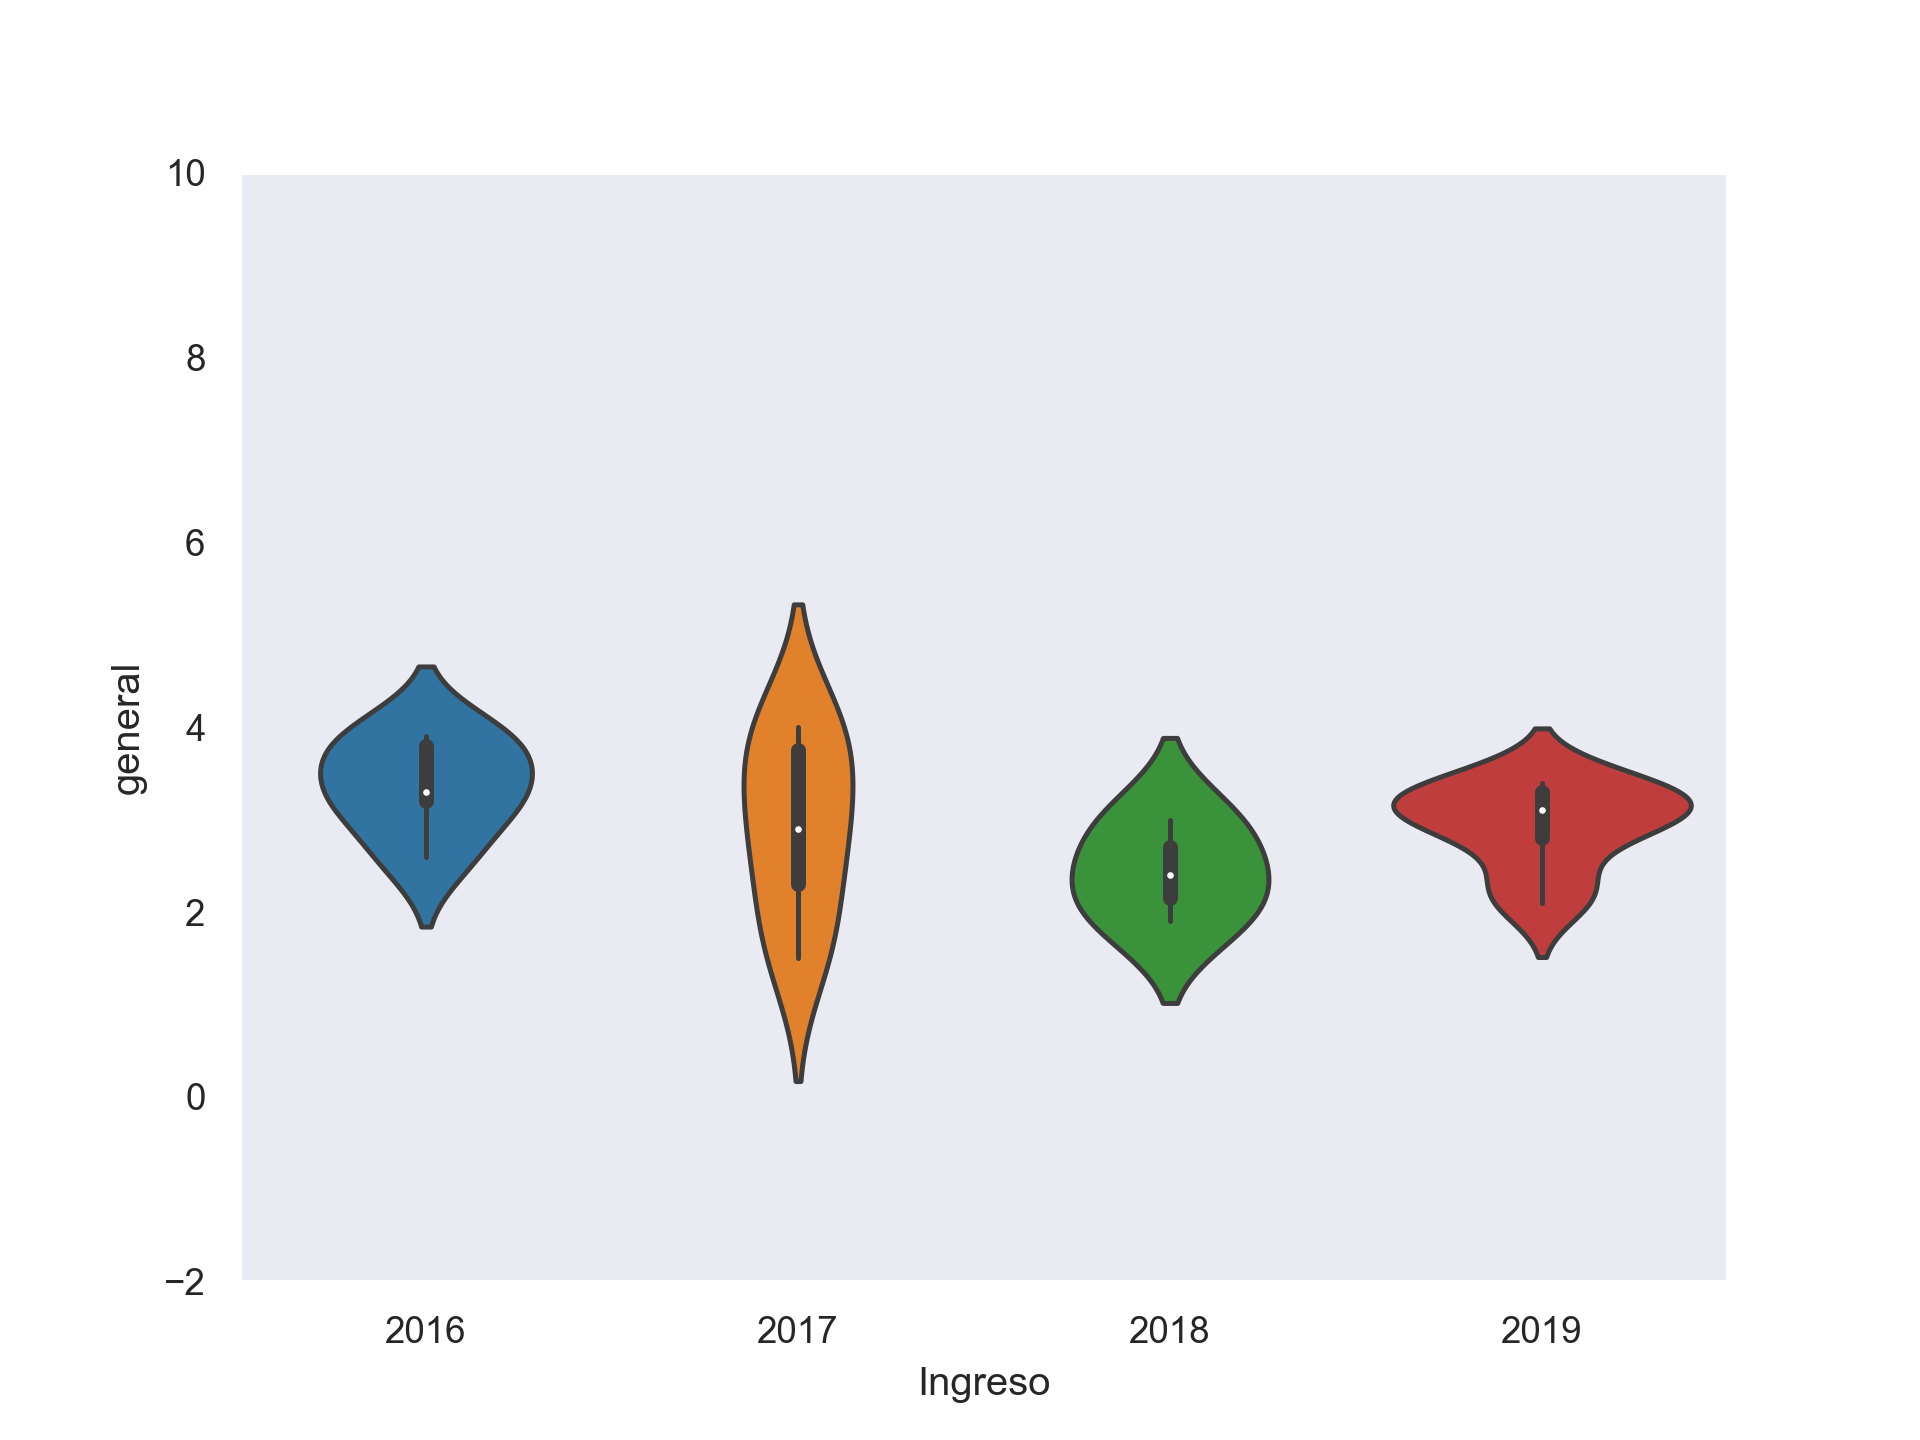
\includegraphics[width=\textwidth]{figuras/figura6.png}
 \caption{Percepción del proceso de escritura, según año de ingreso.}
 \label{fig-percepcion}
 \source{Elaboración propia.}
\end{minipage}
\end{figure}

\subsection{Escritura de código y de textos}

Para evaluar el objetivo de esta investigación, es decir, relacionar las estrategias de producción de código limpio con las concepciones sobre el proceso de escritura en estudiantes de Ingeniería informática se sigue un enfoque relacional basado en la construcción de modelos de predicción de las calificaciones de los estudiantes. En particular, se construyen modelos de regresión lineal que, a partir de las dimensiones de la concepción del proceso de escritura de textos, puedan estimar las calificaciones alcanzadas por los participantes. Debido a que la cohorte ha sido una variable relevante en el desempeño de los estudiantes, se ha decidido incorporar esta dimensión en los modelos predictivos elaborados. 

En la \Cref{fig-modelo1}, se presenta la precisión alcanzada por un modelo de regresión lineal construido a partir de las dimensiones del cuestionario de escritura en conjunto con la variable de cohorte con el propósito de predecir la primera evaluación “Metodologías de resolución de problemas”. Se observa que existe una relación positiva, pero no significativa (r=0.53), entre las concepciones de la escritura y la capacidad para establecer una metodología de resolución de problemas apropiada al dominio del caso de estudio abordado por los estudiantes. 

\begin{figure}[H]
\centering
\begin{minipage}{.75\textwidth}
 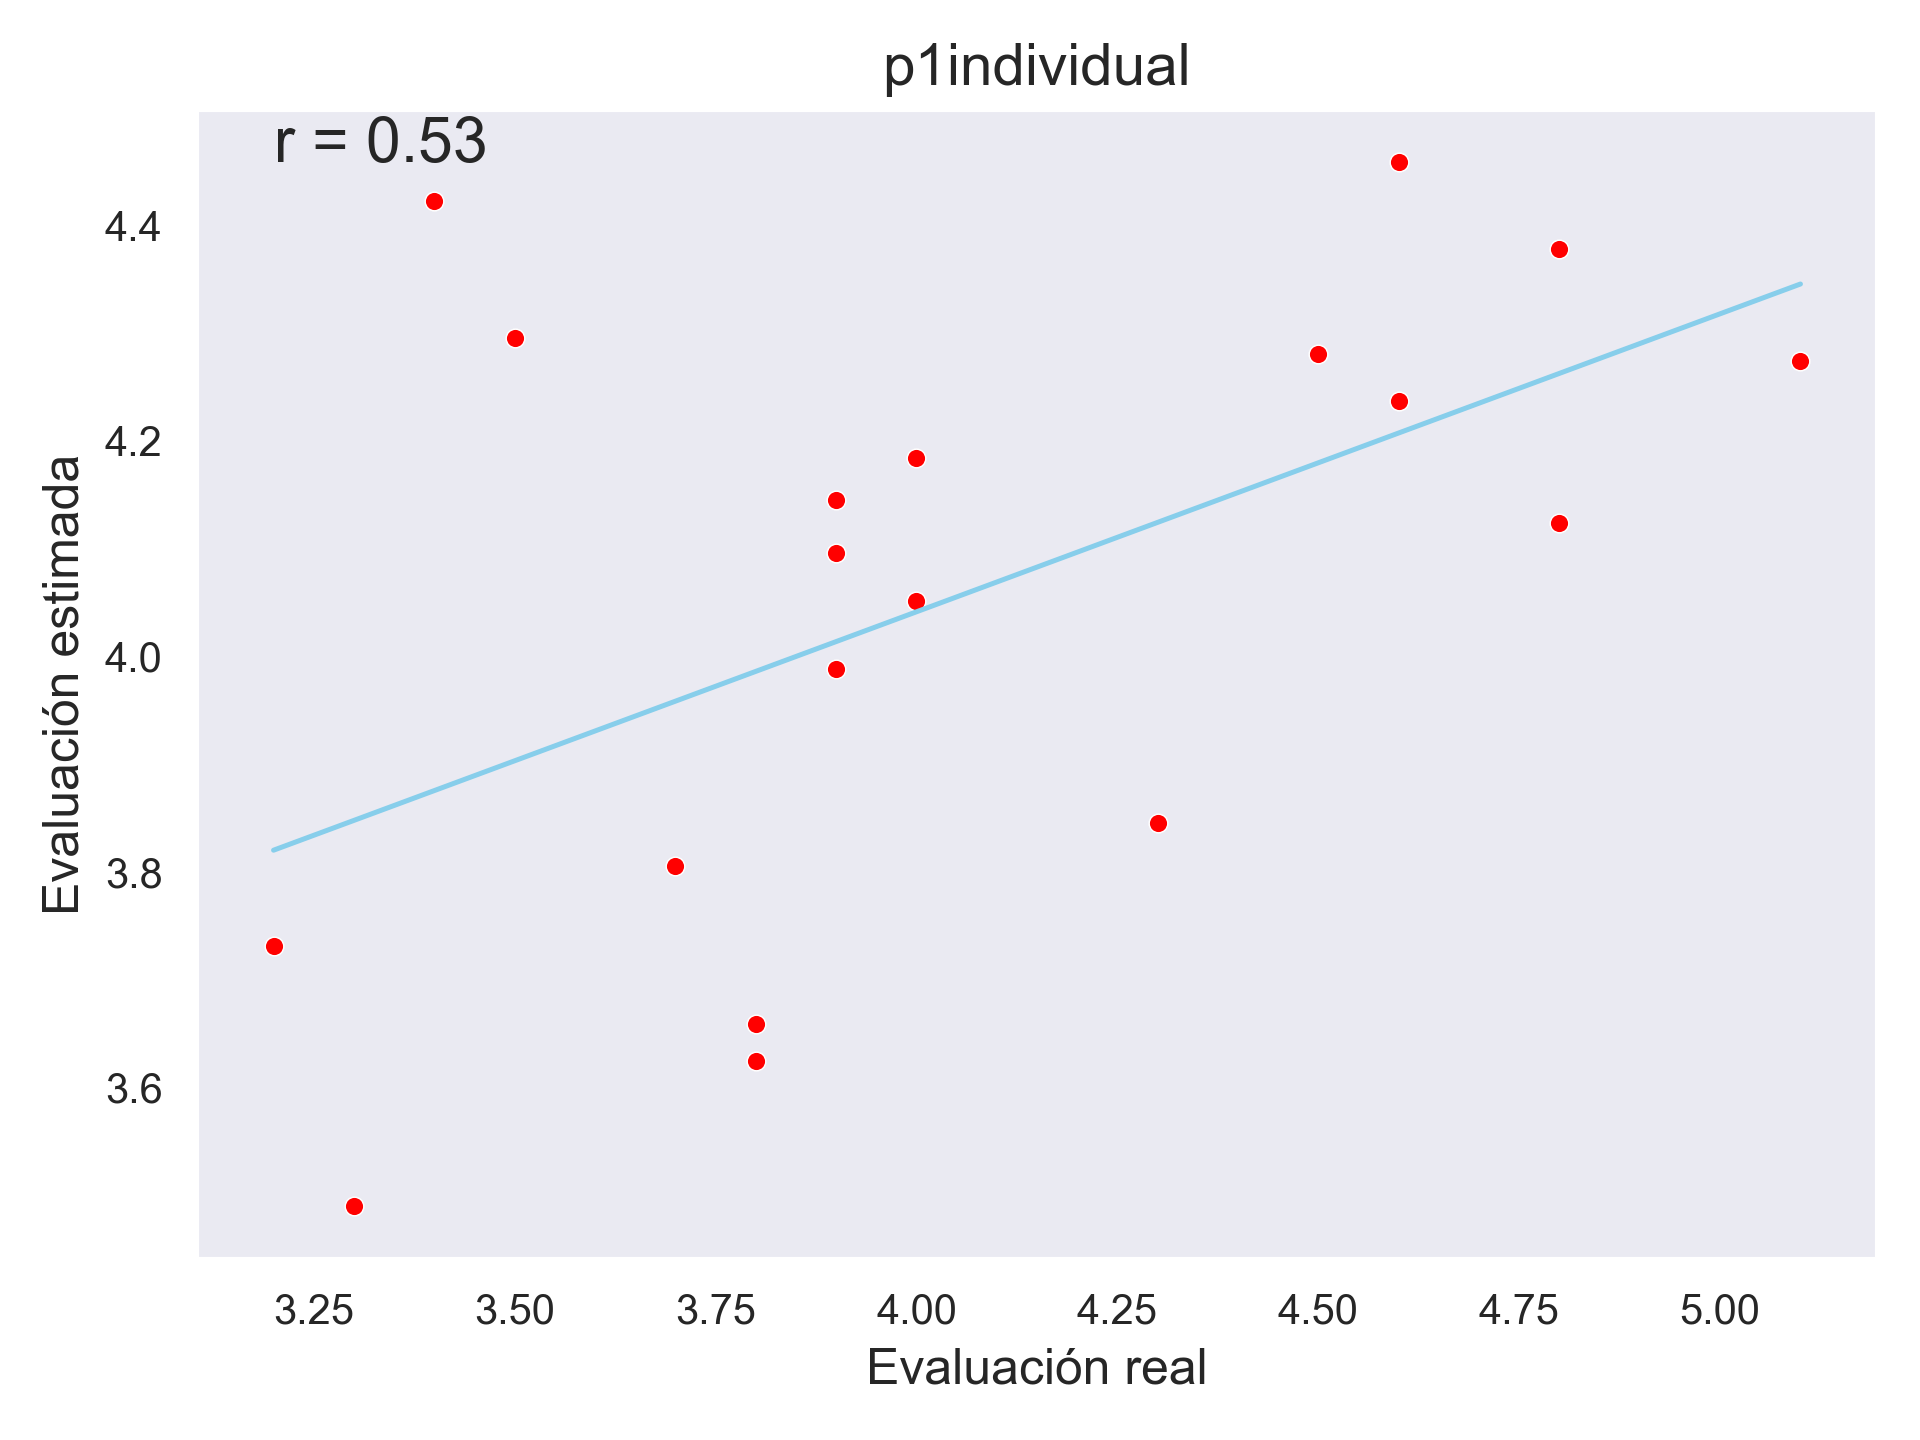
\includegraphics[width=\textwidth]{figuras/figura7.png}
 \caption{Precisión en la estimación del desempeño en la evaluación 1, según dimensiones de concepción de la escritura.}
 \label{fig-modelo1}
 \source{Elaboración propia.}
\end{minipage}
\end{figure}

En la \Cref{fig-modelo2}, se presenta la precisión alcanzada por un modelo de regresión lineal construido a partir de las dimensiones del cuestionario de escritura en conjunto con la variable de cohorte con el fin de predecir los resultados de la segunda evaluación “Codificación limpia”. Se observa que existe una relación positiva mayor al primer modelo y significativa (r=0.75) entre las concepciones de la escritura y la capacidad de producir código limpio por medio de la utilización de buenas prácticas de desarrollo apropiadas al dominio del caso de estudio abordado por los estudiantes. 

\begin{figure}[H]
\centering
\begin{minipage}{.75\textwidth}
 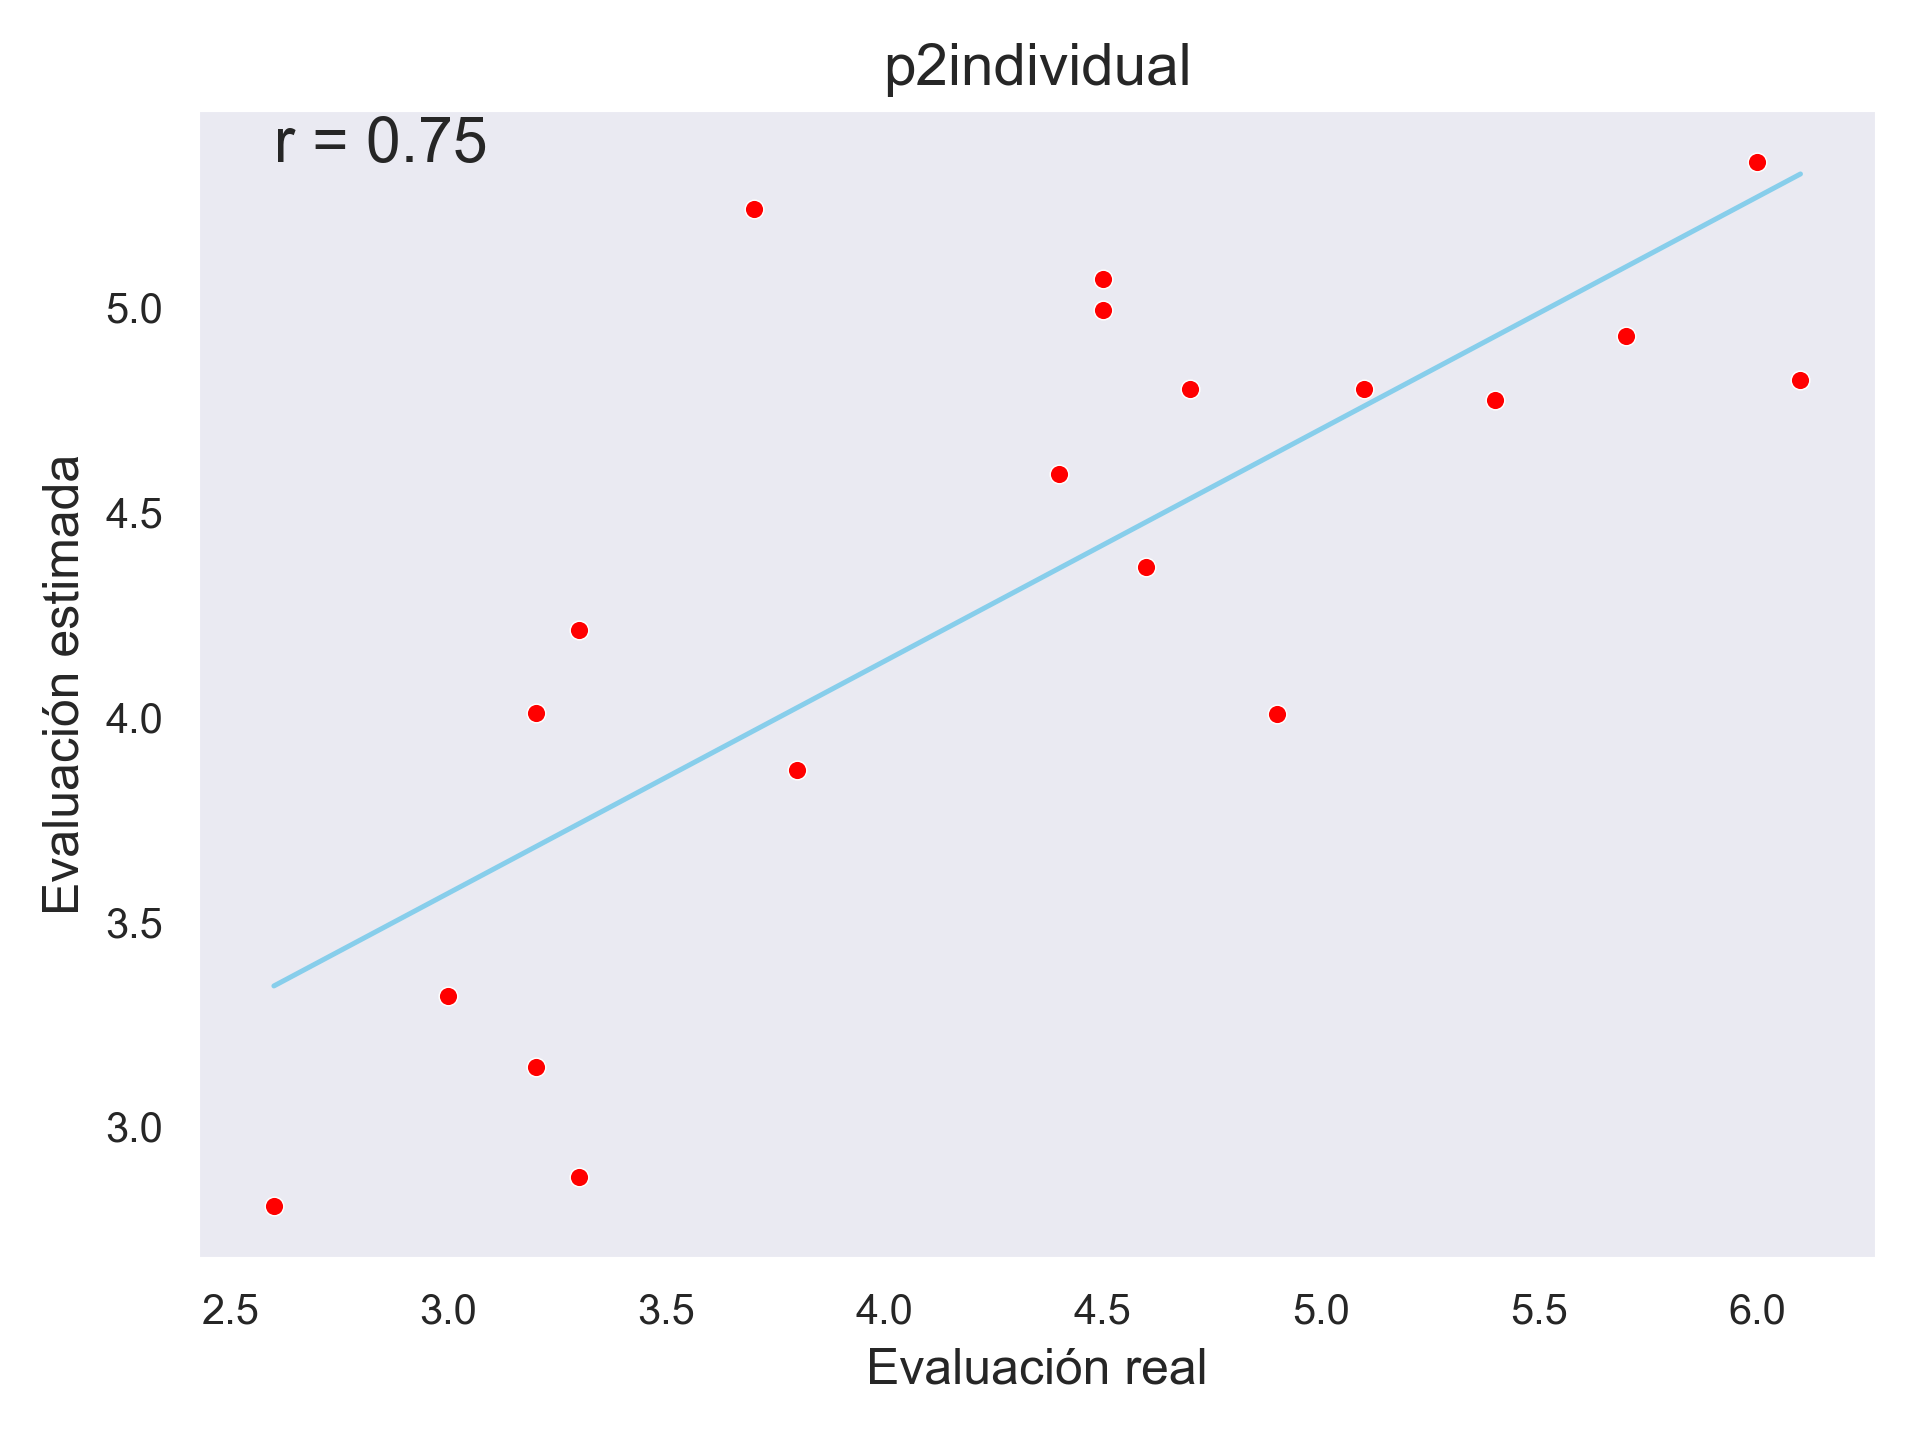
\includegraphics[width=\textwidth]{figuras/figura8.png}
 \caption{Precisión en la estimación del desempeño en la evaluación 2, según dimensiones de concepción de la escritura.}
 \label{fig-modelo2}
 \source{Elaboración propia.}
\end{minipage}
\end{figure}


En la \Cref{fig-modelo3}, se presenta la precisión alcanzada por un modelo de regresión lineal construido a partir de las dimensiones del cuestionario de escritura en conjunto con la variable de cohorte con el fin de predecir los resultados de la tercera evaluación, “Arquitecturas limpias”. Se observa que existe una relación positiva mayor que los dos modelos anteriores y significativa (r=0.87) entre las concepciones de la escritura y la capacidad de producir código limpio por medio de la utilización arquitecturas limpias durante la estimación del esfuerzo de los procesos de desarrollo de software coherentes con el dominio del caso de estudio abordado por los estudiantes. 

\begin{figure}[H]
\centering
\begin{minipage}{.75\textwidth}
 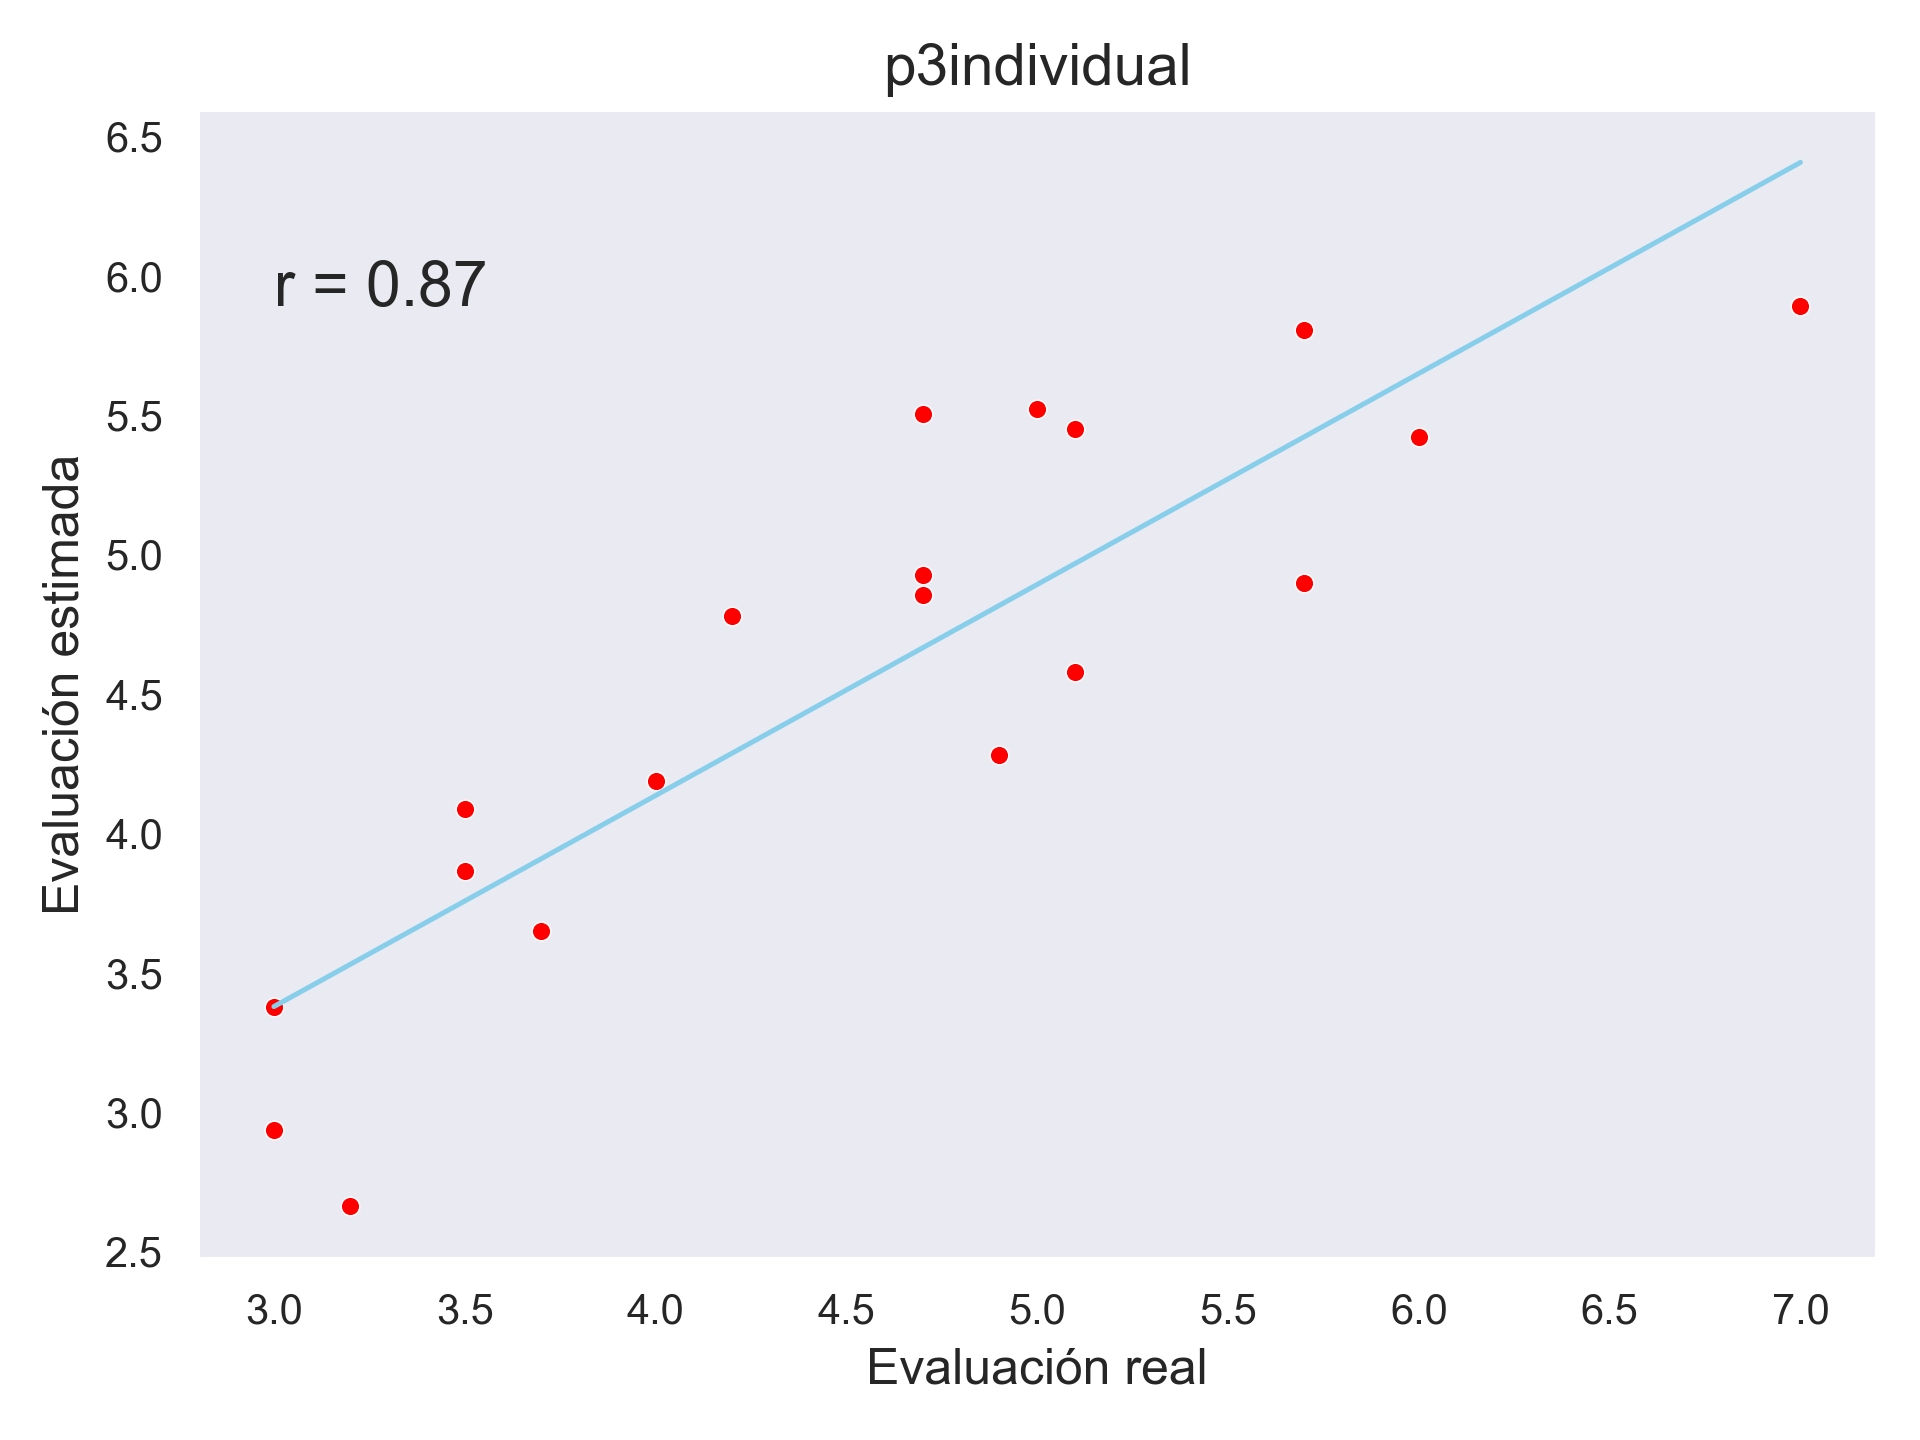
\includegraphics[width=\textwidth]{figuras/figura9.png}
 \caption{Precisión en la estimación del desempeño en la evaluación 3, según dimensiones de concepción de la escritura.}
 \label{fig-modelo3}
 \source{Elaboración propia.}
\end{minipage}
\end{figure}


En consecuencia, los modelos elaborados a partir de las concepciones del proceso de escritura de los estudiantes resultan ser más significativos y precisos cuando las evaluaciones se vinculan con la producción de código, tanto en la segunda como tercera evaluación. Mientras que la evaluación de la resolución de problemas presenta una relación positiva con las concepciones de escritura, no se logran altos niveles de precisión por parte de los modelos de predicción. Finalmente, la introducción de la cohorte como variable predictora genera un mayor nivel de precisión a los modelos elaborados.

\section{Discusión}
Uno de los aspectos más interesantes que surgen desde los resultados, y que está estrechamente vinculado con nuestro objetivo, tiene que ver con cómo varían los desempeños en el ámbito de programación, por una parte, y en el plano de las concepciones sobre la escritura, por otra, en función del año de ingreso. En cuanto a la primera de estas variables, la relación podría explicarse tanto por factores internos como externos. Estudios como el de \textcite{perez2005evolucion} o \textcite{garcia2021transformacion} evidencian no solo la importancia de la motivación en el rendimiento académico, sino también cómo esta tiende a verse mermada con el paso de los cursos académicos, lo que podría explicar el descenso en su desempeño. En cuanto a la escritura, el hecho de que los mejores resultados se hallen en las primeras cohortes (2016 y 2017) puede tener relación con la madurez que en este ámbito se adquiere durante su proceso de formación profesional \cite{valdesleon2022errores}.

En relación con los factores externos que podrían explicar el descenso en el rendimiento en función del año de ingreso, la bibliografía señala que, en muchas ocasiones, los alumnos de cursos terminales suelen asumir compromisos que les demandan mayor tiempo (cargas laborales o familiares), por lo que dedican menos horas semanales a sus estudios \cite{alcover2007analisis, xavier2022persistence}. Sumado a esto, es probable que los cambios en el itinerario formativo de la carrera puedan también incidir en el desempeño, pues se incluyeron, eliminaron y modificaron distintas asignaturas entre los años 2016 y 2022, lo que, de hecho, explica que coincidan en este curso estudiantes de diferentes cohortes.

Además de lo anterior, se observa una mejoría en el rendimiento de la tercera evaluación y, por ende, se estrechan los resultados entre esta dimensión y las percepciones de la escritura durante esta instancia. Uno de los aspectos que podría explicar esto es el hecho de que la evaluación 3 es la que posee un mayor componente procesual, por lo que es lógico pensar que quienes tienen una mirada de la escritura que valora su dimensión  epistémica y compleja tengan mayores habilidades al momento de enfrentar evaluaciones de proceso.  

La relación entre el proceso de escritura de textos y la escritura de código tiene varias similitudes epistemológicas, pero no han sido estudiadas previamente de manera empírica. Esta vinculación permitiría intercambiar y adaptar didácticas pedagógicas para contribuir con la mejora de la enseñanza de la producción tanto de textos como de códigos limpios. En este sentido, hemos analizado la relación empírica entre la percepción del proceso de escritura y las competencias de producción de software en tres etapas evaluativas. En la \Cref{fig-modelo1}, observamos la capacidad que tiene un modelo de regresión lineal de predecir la competencia de los estudiantes vinculada con establecer una metodología de resolución de problemas asociada a un producto de software. Si bien el modelo construido a partir de la percepción de la escritura ha sido capaz de predecir esta competencia de desarrollo, la relación no es significativa. Este resultado puede estar asociado a la estrategia de evaluación, la cual no está orientada a la producción ni de texto ni de código, sino de abstracción y conceptualización del problema.

De igual manera, en la \Cref{fig-modelo2} se presenta un modelo construido con las mismas características de percepción del proceso de escritura, pero con el propósito de predecir la competencia de producir código limpio de una manera ordenada y utilizando estrategias técnicas basadas en patrones. La relación entre ambas dimensiones analizadas es más significativa que la anterior, considerando que, en esta oportunidad, los estudiantes debían producir (escribir) código a partir de un diseño previamente entregado. Luego, en la \Cref{fig-modelo3} se presenta un modelo construido para predecir la competencia de producir código a partir de arquitecturas limpias, donde los estudiantes debían estimar el esfuerzo de escritura de código a partir de una arquitectura de software y, luego, escribir una porción de código. Es decir, los estudiantes debían realizar un proceso completo de producción, desde el diseño abstracto (arquitectura) hasta la codificación de una porción de dicho diseño. En esta oportunidad, la relación observada es aún más significativa que los modelos previos, alcanzado una alta capacidad de predicción del modelo. 
Ahora bien, considerando que esta investigación aborda el campo poco estudiado de la enseñanza de la escritura de código limpio y su relación con el proceso de escritura, resulta necesario reflexionar en torno a las similitudes que existen entre ambos procesos, pues nos parece que poner en diálogo estas disciplinas y su enseñanza puede resultar provechoso para la didáctica de cada una de ellas.  

La didáctica de la escritura ha relevado el carácter procesual que esta posee desde hace ya varias décadas \cite{davoodifard2022overview}. Independientemente del foco que puedan tener los distintos modelos que existen para explicar y enseñar habilidades de escritura, ya sea desde perspectivas cognitivas \cite{flower1996textos} hasta otras de carácter discursivo \cite{bronckart2004actividad}, existe un consenso en que esta debe ser abordada como un proceso y no solo como un producto. 

Así, es innegable que existe una larga tradición en cuanto a los estudios sobre la escritura, estudios que cobran mayor importancia desde la década de los 80’ con los trabajos de \textcite{haves1980identifying}, \textcite{nystrand1982rhetoric}, \textcite{de1984text}, \textcite{bereiter1992modelos}, por nombrar algunos de los más influyentes. Este acervo ha dotado a los estudiosos de la enseñanza de la escritura de un sinnúmero de modelos teóricos y herramientas didácticas que han resultado fundamentales al momento de acompañar procesos de lectoescritura en el aula.

En contraste con esta larga tradición, la enseñanza de la programación ha cobrado especial relevancia en los últimos años, sobre todo debido al interés creciente de incorporar esta disciplina en la formación primaria y secundaria \cite{dapozo2016capacitacion, torrent2019programacion}. Curiosamente, algunas de las experiencias didácticas relacionadas con la enseñanza de la programación suelen presentar aspectos muy cercanos a la didáctica de la escritura, tanto en el metalenguaje utilizado como en la perspectiva procesual de su enseñanza. Un ejemplo de ello es el extensivo uso de la metodología ADRI (Approach, Deployment, Result, and Improvement), la que se define como “an analytical tool which is a well-known quality assurance model for self-review and external review and is used extensively in the education and business sectors” \cite[p.1096]{malik2017model}. Las etapas de esta metodología se presentan a continuación en la \Cref{tabla-modelos}, a la vez que se realiza un paralelo entre estas y la propuesta del grupo Didactext \cite{didactext2003modelo}.

\begin{table}[htpb]
\centering
\begin{threeparttable}
\caption{Comparación modelo ADRI para la enseñanza de la programación con el modelo Didactext para la enseñanza de la escritura.}
\label{tabla-modelos}
\begin{tabular}{ll}
\toprule 
ADRI & Didactext \\ 
\midrule
(1) Approach - Thinking and planning & Acceso al conocimiento y Planificación\\
(2) Deployment - Implementing and doing & Producción textual\\
(3) Results - Monitoring and evaluating & \\
(4) Improvement - Learning and adapting & Revisión\\
\bottomrule
\end{tabular}
\source{Elaboración propia.}
\end{threeparttable}
\end{table}

La \Cref{tabla-modelos} representa una evidencia más de las similitudes que existen entre la enseñanza de una y otra disciplina. Dichas semejanzas van más allá de estos modelos didácticos particulares, pues representan un indicio de la cercanía que existe entre la producción de un código y la producción textual: algunos tecnicismos comunes como sintaxis, estructura, semántica y lenguaje dan cuenta de este vínculo. 
Pese a la relación entre ambas disciplinas y al potencial que esta posee en la enseñanza tanto de la programación como de la escritura, es muy poco lo que se ha publicado sobre ello. Algunos trabajos que abordan dicha cuestión son los de \textcite{santos2020javardise} y \textcite{lindgren2021writing} quienes han esbozado el vínculo entre gramática y texto, y entre la escritura de código y la situación comunicativa, respectivamente. Sin embargo, como resultado de nuestra revisión bibliográfica, no ha sido posible encontrar trabajos que den cuenta de la estrecha relación entre escritura y programación que consideren no solo los aspectos más evidentes (como el metalenguaje común, por ejemplo), sino que indaguen en los procesos sociocognitivos involucrados con el fin de fortalecer su enseñanza.


En consecuencia, la producción de software es un proceso complejo que involucra el análisis del problema a resolver, el diseño de una arquitectura y la producción de código, idealmente, limpio \cite{sommerville2020engineering}. Para ello, es relevante la utilización de patrones o soluciones abstractas recurrentes en la producción de software, las que se encuentran tanto a nivel de diseño como de codificación \cite{wedyan2020impact}. En este trabajo hemos observado cómo este proceso, en cada una de sus etapas, presenta una relación positiva con la percepción del proceso de escritura por parte de los estudiantes. En particular, cuando el proceso de producción de software se lleva a cabo de manera completa, la relación entre estas dos dimensiones de análisis se robustece (\Cref{fig-modelo2}).

\section{Conclusiones}

El objetivo de este trabajo fue relacionar la producción de código limpio con las concepciones sobre el proceso de escritura en estudiantes de Ingeniería informática. De esta forma, gracias a las tres evaluaciones prácticas que dieron seguimiento al proceso de producción de código limpio y al cuestionario sobre percepciones acerca de la escritura, se logró identificar tres aspectos clave:
\begin{enumerate*}[label=\arabic*)]
    \item la incidencia del año de ingreso en el desempeño académico,
    \item la relación positiva entre producción de código limpio y percepciones sobre la escritura y las que se orientan hacia el desarrollo de competencias escritas y
    \item las similitudes entre las propuestas didácticas para la enseñanza de la programación. 
\end{enumerate*}

Respecto del primer hallazgo, a saber, la relación entre rendimiento y año de ingreso, la revisión bibliográfica señala que tanto factores personales como académicos pueden haber incidido en esto, aunque resulta necesario seguir indagando con el fin de dar respuesta ante esta necesidad formativa. Luego, en cuanto a la relación entre la producción de código limpio y las percepciones sobre el proceso de escritura, hemos identificado que existe una correlación significativa entre ambas variables, lo que podría explicarse debido a las similitudes que existen entre ambos procesos, tanto a nivel cognitivo como en el ámbito de su enseñanza. 

Si bien el diseño y las características del estudio no permiten generalizar los resultados, estos invitan a profundizar en una interesante línea de investigación que se oriente hacia la didáctica, que permita nutrir los procesos de enseñanza-aprendizaje de ambas disciplinas y que considere los aspectos epistémicos, sociocognitivos, procesuales y socioafectivos presentes tanto en el aprendizaje de la programación como en el de la escritura.


\printbibliography\label{sec-bib}
% if the text is not in Portuguese, it might be necessary to use the code below instead to print the correct ABNT abbreviations [s.n.], [s.l.]
%\begin{portuguese}
%\printbibliography[title={Bibliography}]
%\end{portuguese}


%full list: conceptualization,datacuration,formalanalysis,funding,investigation,methodology,projadm,resources,software,supervision,validation,visualization,writing,review
\begin{contributors}[sec-contributors]
\authorcontribution{Cristian Olivares-Rodríguez}[conceptualization,datacuration,formalanalysis,software,validation]
\authorcontribution{Gabriel Valdés-León}[conceptualization,formalanalysis,methodology,validation]
\authorcontribution{Martha Vidal-Sepúlveda}[conceptualization,visualization,writing,review]
\authorcontribution{Romina Oyarzún-Yañez}[conceptualization,visualization,writing,review]

\end{contributors}




\end{document}

